\section{Parallel Machine Models} \label{sec:6}

\subsection{Makespan without Preemptions} \label{subsec:6.1}

\subsubsection{List Scheduling and Longest Processing Time} \label{subsubsec:6.1.1}
The makespan is not a very interesting objective for a single machine. 
However, for parallel machine models, minimizing the makespan has the effect 
of balancing the load over the various machines, which is an important 
objective in practice. Recall that we denote this by $(P_m~\|~C_{\max})$.

One can see that $(P_2~\|~C_{\max})$ is $\NP$-hard via a reduction from 
\textsc{Partition}. Indeed, consider an instance of \textsc{Partition}, 
where we are given $a_1, \dots, a_t \in \Z^+$ and want to find a subset 
$S \subseteq \{1, \dots, t\}$ such that 
\[ \sum_{j\in S} a_j = \frac12 \sum_{j=1}^t a_j = b. \] 
Let $n = t$ be the number of jobs each with processing time $p_j = a_j$. Then 
it is easy to check that there is a schedule with optimal value at most 
$\frac12 \sum_{j=1}^n p_j$ if and only if there is a solution to the 
\textsc{Partition} instance. 

Over the years, there have been many heuristics developed for 
$(P_m~\|~C_{\max})$. We focus on one such heuristic, and present it by 
discussing some history on how this algorithm was developed. First, we 
take a look at the list scheduling rule, which runs in $O(n\log m)$ time 
using a priority queue for the loads. 

\begin{algo}[List Scheduling]{algo:6.1}
    Given $n$ jobs in some arbitrary order, assign job $j$ to machine $i$ 
    whose load is smallest so far for each $j \in [n]$. 
\end{algo}

There are two obvious lower bounds on OPT, namely 
\begin{enumerate}[(1)]
    \item $\text{OPT} \geq \max_{j\in[n]} p_j$ since the jobs are not preemptive, and 
    \item $\text{OPT} \geq \frac1m \sum_{j=1}^n p_j$ because at least one machine must 
    have load which is at least the average. 
\end{enumerate}
We shall denote the load of a machine $i$ by $L(i) = p(S(i)) = 
\sum_{j\in S(i)} p_j$, where $S(i)$ is the set of jobs assigned to machine $i$.

\begin{theo}{theo:6.2}
    Algorithm~\ref{algo:6.1} is a $2$-approximation for $(P_m~\|~C_{\max})$. 
\end{theo}
\begin{pf}
    Let $i$ denote the machine which the highest load determining the objective 
    value. Let $j$ be the last job scheduled on machine $i$. When job $j$ was 
    assigned to machine $i$, it had the smallest load. Its load before the 
    assignment was $L(i) - p_j$, and thus $L(i) - p_j \leq L(k)$ for all 
    $1 \leq k \leq m$. Summing up this inequality over all $k$ and 
    dividing by $m$, we obtain 
    \[ L(i) - p_j \leq \frac1m \sum_{k=1}^m L(k) = \frac1m \sum_{j=1}^n p_j 
    \leq \text{OPT}. \] 
    We deduce that $L(i) = (L(i) - p_j) + p_j \leq 2 \cdot \text{OPT}$. 
\end{pf}

Is this analysis tight? That is, are there any examples where the factor 
is as bad as $2$? The answer is essentially yes. Suppose there are $m$ machines.
Take $m(m-1)$ jobs each with processing time $1$, and let the last job 
in the order have processing time $m$. Then the list scheduling algorithm 
will try to balance the $m(m-1)$ jobs among the $m$ machines first. Then 
we are forced to run the last job with processing time $m$ last on one 
of the machines, and that machine has load $2m - 1$. An optimal schedule 
instead places the job with processing time $m$ on its own machine, 
and balances the load of the $m(m-1)$ jobs between the remaining $m-1$ 
machines. This gives a makespan of $m$ instead. 

It can be shown that Algorithm~\ref{algo:6.1} is in fact a 
$(2 - \frac1m)$-approximation, and the above example shows that this is 
exactly a tight bound. 

We now consider the {\bf Longest Processing Time first (LPT)} rule.

\begin{algo}[LPT]{algo:6.3}
    Sort the $n$ jobs in decreasing order of $p_j$, then run 
    Algorithm~\ref{algo:6.1}.
\end{algo}

This is equivalent to the following procedure: at time $t = 0$, 
assign the $m$ longest jobs to the $m$ machines. Afterwards, 
whenever a machine is freed, the longest job among those not yet processed is 
put on the machine. This heuristic tries to place the shorter jobs more towards 
the end of the schedule, where they can be used for balancing the loads.

\begin{exercise}{exercise:6.4}
    Show that if an optimal schedule results in at most two jobs on any
    machine, then LPT is optimal.
\end{exercise}

Under the LPT rule in the case that $n \geq m+1$, we also have an additional 
lower bound on OPT. This is given by $\text{OPT} \geq 2p_{m+1}$ because 
at least one machine must run two jobs by the time it gets to the 
$(m+1)$-th job, and that machine has load at least $2p_{m+1}$ as the 
jobs are in decreasing order of the processing times. 

\begin{theo}{theo:6.5}
    Algorithm~\ref{algo:6.3} is a $\frac32$-approximation for $(P_m~\|~C_{\max})$.
\end{theo}
\begin{pf}
    This is the same proof as Theorem~\ref{theo:6.2}, except that we now 
    have $p_j \leq p_{m+1} \leq \text{OPT}/2$. 
\end{pf}

This is actually a very crude bound. We give a more sophisticated analysis 
showing that the LPT rule is a $(\frac43 - \frac{1}{3m})$-approximation, 
and that this bound is tight.  

\begin{theo}{theo:6.6}
    For $(P_m~\|~C_{\max})$, we have 
    \[ \frac{C_{\max}(\text{LPT})}{C_{\max}(\text{OPT})} \leq 
    \frac43 - \frac{1}{3m}. \] 
\end{theo}
\begin{pf}
    We proceed by contradiction. Suppose there are counterexamples with 
    ratio strictly larger than $\frac43 - \frac1{3m}$. Among these 
    counterexamples, there must be a counterexample with the least 
    number of jobs. 

    Suppose this smallest counterexample has $n$ jobs. This counterexample 
    has a useful property: under LPT, the shortest job is the last job 
    to start its processing and also the last job to finish its processing. 
    To see why this is true, note that by the definition of LPT, 
    the shortest job is the last to finish its processing. On the other hand, 
    if this job was not last to finish processing, then the deletion of 
    this smallest job would result in a counterexample with fewer jobs since 
    $C_{\max}(\text{LPT})$ remains the same while $C_{\max}(\text{OPT})$ 
    either stays the same or decreases, which is a contradiction to our 
    assumption that our counterexample was minimal. 

    Therefore, for our smallest counterexample, the starting time of the 
    shortest job is $C_{\max}(\text{LPT}) - p_n$. At this point, all other 
    machines are busy, so we have 
    \[ C_{\max}(\text{LPT}) - p_n \leq \frac1m \sum_{j=1}^{n-1} p_j. \] 
    The right-hand side is an upper bound on the starting time of the 
    shortest job, and is achieved when scheduling the first $n-1$ jobs 
    according to LPT results in each machine having exactly the same 
    amount of processing to do. Then we have 
    \[ C_{\max}(\text{LPT}) \leq p_n + \frac1m \sum_{j=1}^{n-1} p_j 
    = p_n\left(1 - \frac1m \right) + \frac1m \sum_{j=1}^n p_j. \] 
    We also know that $C_{\max}(\text{OPT}) \geq \frac1m \sum_{j=1}^n p_j$, 
    so for the counterexample, we obtain 
    \[ \frac43 - \frac1{3m} < \frac{C_{\max}(\text{LPT})}{C_{\max}(\text{OPT})} 
    \leq \frac{p_n(1 - \frac1m) + \frac1m \sum_{j=1}^n p_j}{C_{\max}(\text{OPT})} 
    \leq \frac{p_n(1 - \frac1m)}{C_{\max}(\text{OPT})} + 1. \] 
    Rearranging gives us $C_{\max}(\text{OPT}) < 3p_n$. Note that this 
    is a strict inequality. Since $p_n$ is the shortest job, this implies that 
    for the smallest counterexample, the optimal schedule results in at 
    most two jobs on each machine. But by Exercise~\ref{exercise:6.4}, 
    LPT is optimal under this condition, which is a contradiction. 
\end{pf}

\begin{exmp}{exmp:6.7}
    We consider an example where LPT performs very badly and attains the 
    worst case bound. Suppose there are $m = 4$ parallel machines with the 
    following $n = 9$ jobs. 
    \begin{align*}
        \begin{array}{c|ccccccccc}
            j & 1 & 2 & 3 & 4 & 5 & 6 & 7 & 8 & 9 \\ \hline 
            p_j & 7 & 7 & 6 & 6 & 5 & 5 & 4 & 4 & 4
        \end{array}
    \end{align*}
    Then the following schedule is optimal with $C_{\max} = 12$.
    \begin{center} 
        \begin{tikzpicture}[/pgfgantt/y unit chart=0.7cm] 
            \begin{ganttchart}[
                title/.style={draw=none},
                canvas/.append style={draw=none}, 
                bar top shift=0.1, bar height=0.6,
                y unit title=0.7cm,
            ]{1}{12}
                \ganttbar{Machine 1}{1}{7} \ganttbar[inline]{7}{1}{7} \ganttbar[inline]{5}{8}{12} \\ 
                \ganttbar{Machine 2}{1}{7} \ganttbar[inline]{7}{1}{7} \ganttbar[inline]{5}{8}{12} \\ 
                \ganttbar{Machine 3}{1}{6} \ganttbar[inline]{6}{1}{6} \ganttbar[inline]{6}{7}{12} \\ 
                \ganttbar{Machine 4}{1}{4} \ganttbar[inline]{4}{1}{4} \ganttbar[inline]{4}{5}{8} \ganttbar[inline]{4}{9}{12} \\
                \gantttitlelist{1,...,12}{1}
            \end{ganttchart}
        \end{tikzpicture}
    \end{center}
    \vspace{-0.4cm}
    On the other hand, LPT gives the following schedule which has $C_{\max} = 15$, 
    which is the worst case we could possibly have from Theorem~\ref{theo:6.6}.
    \begin{center} 
        \begin{tikzpicture}[/pgfgantt/y unit chart=0.7cm] 
            \begin{ganttchart}[
                title/.style={draw=none},
                canvas/.append style={draw=none}, 
                bar top shift=0.1, bar height=0.6,
                y unit title=0.7cm,
            ]{1}{12}
                \ganttbar{Machine 1}{1}{7} \ganttbar[inline]{7}{1}{7} \ganttbar[inline]{4}{8}{11} \ganttbar[inline]{4}{12}{15} \\ 
                \ganttbar{Machine 2}{1}{7} \ganttbar[inline]{7}{1}{7} \ganttbar[inline]{4}{8}{11} \\ 
                \ganttbar{Machine 3}{1}{6} \ganttbar[inline]{6}{1}{6} \ganttbar[inline]{5}{7}{11} \\ 
                \ganttbar{Machine 4}{1}{6} \ganttbar[inline]{6}{1}{6} \ganttbar[inline]{5}{7}{11} \\
                \gantttitlelist{1,...,15}{1}
            \end{ganttchart}
        \end{tikzpicture}
    \end{center}
    \vspace{-0.4cm}
\end{exmp}

\subsubsection{Makespan with Precedence Constraints} \label{subsubsec:6.1.2}
Now, consider the same problem with the jobs subject to precedence constraints,
namely $(P_m~|~\text{prec}~|~C_{\max})$. From a complexity point of view, this 
problem has to be at least as hard as the problem without precedence constraints.
In particular, it can be shown that $(P_m~|~\text{prec}~|~C_{\max})$ is 
strongly $\NP$-hard for $2 \leq m < n$, even in the case where the precedence 
constraints are chains. To obtain some insight into the effects of precedence 
constraints, we consider a number of special cases. 

Suppose there are an unlimited number of machines in parallel, or that 
$m \geq n$ so the number of machines is at least as large as the number of jobs.
We can denote this problem by $(P_\infty~|~\text{prec}~|~C_{\max})$. This 
is a classical problem in the field of project planning, and its study 
has led to the development of the well-known {\bf Critical Path Method 
(CPM)} and {\bf Project Evaluation Review Technique (PERT)}. In this case, 
the optimal schedule and the minimum makespan are determined by a very simple 
algorithm. 

\begin{algo}[Minimizing the Makespan of a Project]{algo:6.8}
    Schedule the jobs one at a time starting at time zero. Whenever a job has 
    been completed, start all jobs of in which all predecessors have been 
    completed (that is, the set of all schedulable jobs).
\end{algo}

So $(1~|~\text{prec}~|~C_{\max})$ and $(P_\infty~|~\text{prec}~|~C_{\max})$,
are easy. But we stated earlier that $(P_m~|~\text{prec}~|~C_{\max})$ is 
strongly $\NP$-hard for $2 \leq m < n$. Even $(P_m~|~p_j = 1, \text{prec}~|~C_{\max})$,
where the processing times are all unit, is not easy. However, by constraining 
the problem further and assuming that the precedence graph takes the form 
of a tree (either an intree or an outtree), the problem $(P_m~|~p_j = 1, 
\text{tree}~|~C_{\max})$ is easily solvable. This leads to the well-known 
scheduling rule known as the {\bf Critical Path (CP)} rule. 

\begin{algo}[Critical Path (CP)]{algo:6.9}
    The job at the head of the longest string of jobs in the precedence
    constraints graph has the highest priority. Ties can be broken arbitrarily.
\end{algo}

We also consider a different priority rule that considers the largest 
total number of successors (not just the immediate successors) in the 
precedence graph. This is called the {\bf Largest Number of Successors first 
(LNS)} rule. 

\begin{algo}[Largest Number of Successors first (LNS)]{algo:6.10}
    The job with the largest total number of successors in the 
    precedence graph has the highest priority. Ties can be broken arbitrarily.
\end{algo}

Note that the LNS rule is equivalent to the CP rule when the precedence 
graph takes the form of chains or an intree. It can also be shown that 
LNS is optimal for outtrees, and thus LNS is also optimal for 
$(P_m~|~p_j = 1, \text{tree}~|~C_{\max})$.

We will not prove the optimality of the CP and LNS rules for 
$(P_m~|~p_j = 1, \text{tree}~|~C_{\max})$. But how do these rules perform for 
arbitrary precedence constraints when all processing times are equal to $1$? 

In the case where there are two parallel machines, it can be shown that 
\[ \frac{C_{\max}(\text{CP})}{C_{\max}(\text{OPT})} \leq \frac43. \] 
When there are more than two parallel machines, the worst case ratio is larger. 
We show that the worst case bound can be reached for two machines in the 
following example. 

\begin{exmp}{exmp:6.11}
    Consider the instance of $(P_2~|~p_j=1, \text{prec}~|~C_{\max})$ 
    with precedence constraints given by the following directed acyclic 
    graph. 
    \begin{center}
        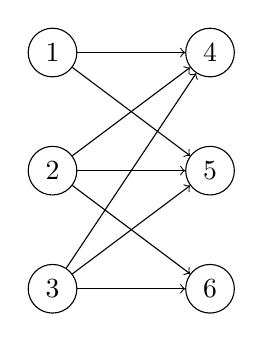
\begin{tikzpicture}              
            \node [circle, draw=black] (1) at (0, 3) {$1$};  
            \node [circle, draw=black] (2) at (0, 1.5) {$2$}; 
            \node [circle, draw=black] (3) at (0, 0) {$3$}; 
            \node [circle, draw=black] (4) at (2, 3) {$4$}; 
            \node [circle, draw=black] (5) at (2, 1.5) {$5$}; 
            \node [circle, draw=black] (6) at (2, 0) {$6$};

            \draw [->] (1) -- (4); \draw [->] (1) -- (5); 
            \draw [->] (2) -- (4); \draw [->] (2) -- (5); \draw [->] (2) -- (6);
            \draw [->] (3) -- (4); \draw [->] (3) -- (5); \draw [->] (3) -- (6);        
        \end{tikzpicture} 
    \end{center}
    This is almost a complete bipartite graph; it is only missing the edge 
    from job $1$ to job $6$. An optimal schedule is given below with 
    $C_{\max} = 3$. 
    \begin{center} 
        \begin{tikzpicture}[/pgfgantt/y unit chart=0.7cm] 
            \begin{ganttchart}[
                title/.style={draw=none},
                canvas/.append style={draw=none}, 
                bar top shift=0.1, bar height=0.6,
                y unit title=0.7cm,
            ]{1}{3}
                \ganttbar{Machine 1}{1}{2} \ganttbar[inline]{2}{1}{1} \ganttbar[inline]{1}{2}{2} \ganttbar[inline]{4}{3}{3} \\ 
                \ganttbar{Machine 2}{1}{2} \ganttbar[inline]{3}{1}{1} \ganttbar[inline]{6}{2}{2} \ganttbar[inline]{5}{3}{3}
            \end{ganttchart}
        \end{tikzpicture}
    \end{center}
    \vspace{-0.4cm}
    On the other hand, the CP rule could arbitrarily pick job $1$ to 
    be processed at time $0$, which would prevent job $6$ from running 
    at time $1$ as its predecessors are jobs $2$ and $3$. One such schedule 
    obtained from the CP rule is as follows, and it has $C_{\max} = 4$, 
    which matches the worst case bound above. 
    \begin{center} 
        \begin{tikzpicture}[/pgfgantt/y unit chart=0.7cm] 
            \begin{ganttchart}[
                title/.style={draw=none},
                canvas/.append style={draw=none}, 
                bar top shift=0.1, bar height=0.6,
                y unit title=0.7cm,
            ]{1}{3}
                \ganttbar{Machine 1}{1}{1} \ganttbar[inline]{1}{1}{1} \ganttbar[inline]{3}{2}{2} \ganttbar[inline]{4}{3}{3} \ganttbar[inline]{6}{4}{4} \\ 
                \ganttbar{Machine 2}{1}{1} \ganttbar[inline]{2}{1}{1} \ganttbar[inline]{5}{3}{3} 
            \end{ganttchart}
        \end{tikzpicture}
    \end{center}
\end{exmp}

Next, we give an example where LNS does not yield an optimal schedule for 
arbitrary precedence constraints. 

\begin{exmp}{exmp:6.12}
    Consider the instance of $(P_2~|~p_j=1, \text{prec}~|~C_{\max})$ 
    with precedence constraints given by the following directed acyclic 
    graph. 
    \begin{center}
        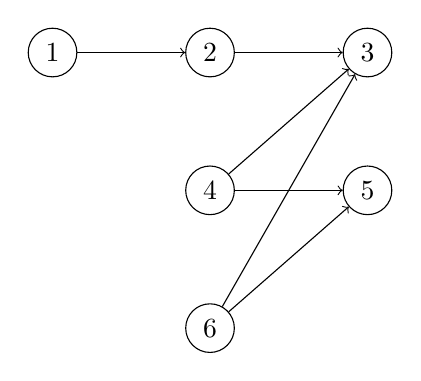
\begin{tikzpicture}              
            \node [circle, draw=black] (1) at (0, 3.5) {$1$};  
            \node [circle, draw=black] (2) at (2, 3.5) {$2$}; 
            \node [circle, draw=black] (3) at (4, 3.5) {$3$}; 
            \node [circle, draw=black] (4) at (2, 1.75) {$4$}; 
            \node [circle, draw=black] (5) at (4, 1.75) {$5$}; 
            \node [circle, draw=black] (6) at (2, 0) {$6$};

            \draw [->] (1) -- (2); \draw [->] (2) -- (3); 
            \draw [->] (4) -- (3); \draw [->] (4) -- (5);
            \draw [->] (6) -- (3); \draw [->] (6) -- (5);     
        \end{tikzpicture} 
    \end{center}
    \newpage
    An optimal schedule is given below with $C_{\max} = 3$. 
    \begin{center} 
        \begin{tikzpicture}[/pgfgantt/y unit chart=0.7cm] 
            \begin{ganttchart}[
                title/.style={draw=none},
                canvas/.append style={draw=none}, 
                bar top shift=0.1, bar height=0.6,
                y unit title=0.7cm,
            ]{1}{3}
                \ganttbar{Machine 1}{1}{2} \ganttbar[inline]{1}{1}{1} \ganttbar[inline]{2}{2}{2} \ganttbar[inline]{3}{3}{3} \\ 
                \ganttbar{Machine 2}{1}{2} \ganttbar[inline]{4}{1}{1} \ganttbar[inline]{6}{2}{2} \ganttbar[inline]{5}{3}{3}
            \end{ganttchart}
        \end{tikzpicture}
    \end{center}
    \vspace{-0.4cm}
    The LNS rule would pick jobs $4$ and $6$ first as they each have two 
    successors. This causes job $2$ to finish at time $3$ at the earliest, 
    preventing job $3$ from being run afterwards. So the LNS rule 
    yields a schedule with $C_{\max} = 4$. 
    \begin{center} 
        \begin{tikzpicture}[/pgfgantt/y unit chart=0.7cm] 
            \begin{ganttchart}[
                title/.style={draw=none},
                canvas/.append style={draw=none}, 
                bar top shift=0.1, bar height=0.6,
                y unit title=0.7cm,
            ]{1}{3}
                \ganttbar{Machine 1}{1}{2} \ganttbar[inline]{4}{1}{1} \ganttbar[inline]{1}{2}{2} \ganttbar[inline]{2}{3}{3} \ganttbar[inline]{3}{4}{4} \\ 
                \ganttbar{Machine 2}{1}{2} \ganttbar[inline]{6}{1}{1} \ganttbar[inline]{5}{2}{2} 
            \end{ganttchart}
        \end{tikzpicture}
    \end{center}
    \vspace{-0.4cm}
\end{exmp}

Both the CP rule and the LNS rule have more generalized versions that
can be applied to problems with arbitrary job processing times. Instead of
counting the number of jobs (as in the case with unit processing times), these
more generalized versions prioritize based on the total amount of processing
remaining to be done on the jobs in question. The CP rule then gives the
highest priority to the job that is heading the string of jobs with the largest
total amount of processing (with the processing time of the job itself also being
included in this total). The generalization of the LNS rule gives the highest
priority to that job that precedes the largest total amount of processing; again
the processing time of the job itself is also included in the total. The LNS name
is clearly not appropriate for this generalization with arbitrary processing times,
as it refers to a number of jobs rather than to a total amount of processing.

\subsubsection{Makespan with Machine Dependent Constraints} \label{subsubsec:6.1.3}
We consider another generalization of the $(P_m~||~C_{\max})$ problem 
where each job $j$ is only allowed to be run on a subset $M_j$ of the $m$ 
parallel machines. We will again consider the case with unit processing times, 
denoted by $(P_m~|~p_j=1, M_j~|~C_{\max})$. 

We note that this problem can be represented using a bipartite graph with $n$ 
edges $1, \dots, n$ corresponding to the jobs and $m$ edges $\text{mc}_1, 
\dots, \text{mc}_m$ corresponding to the machines. We place an edge 
$(j, \text{mc}_i)$ in the graph if and only if $i \in M_j$. 

We say that the sets $M_j$ are {\bf nested} if exactly one of the 
following conditions hold for any two jobs $j$ and $k$: 
\begin{enumerate}[(i)]
    \item $M_j = M_k$; 
    \item $M_j \subsetneq M_k$;
    \item $M_k \subsetneq M_j$; or 
    \item $M_j \cap M_k = \varnothing$.
\end{enumerate} 
When the sets $M_j$ are nested, the {\bf Least Flexible Job (LFJ)} rule 
plays an important role. 

\begin{algo}[Least Flexible Job (LFJ)]{algo:6.13}
    Every time a machine is freed, select among the available jobs the job 
    that can be processed on the \emph{smallest} number of machines. Ties 
    can be broken arbitrarily. 
\end{algo}

This rule is rather crude as it does not specify, for example, which
machine should be considered first when several machines become available at
the same time. It can be shown that the LFJ rule is optimal for 
$(P_m~|~p_j=1, M_j~|~C_{\max})$ when the sets $M_j$ are nested by using 
a standard interchange argument. In particular, when there are two 
machines, the sets $M_j$ are always nested, so the LFJ rule is optimal 
for $(P_2~|~p_j=1, M_j~|~C_{\max})$. However, in the case that $m \geq 3$ 
and the sets $M_j$ are arbitrary, the LFJ rule will not always yield an 
optimal schedule. We give an example of this below. 

\begin{exmp}{exmp:6.14}
    Consider the following instance of $(P_4~|~p_j=1, M_j~|~C_{\max})$ 
    with $n = 8$ jobs. 
    \begin{align*}
        \begin{array}{c|cccccccc}
            j & 1 & 2 & 3 & 4 & 5 & 6 & 7 & 8 \\ \hline 
            M_j & \{1,2\} & \{1,3,4\} & \{1,3,4\} & \{2\} & \{3,4\} 
            & \{3,4\} & \{3,4\} & \{3,4\}
        \end{array}
    \end{align*}
    It is clear that the sets $M_j$ are not nested by considering $M_1$ 
    and $M_2$. We now run the LFJ rule. Consider machine $1$ first. 
    The least flexible job that can be processed on machine $1$ is job $1$ 
    since it can be processed on only two machines, while jobs $2$ and $3$ 
    can be processed on three machines. The least flexible job to be processed 
    on machine $2$ is clearly job $4$. At time $0$, the least flexible jobs 
    to be processed on machines $3$ and $4$ could be jobs $5$ and $6$. 
    At time $1$, after jobs $1$, $4$, $5$, and $6$ have completed their processing 
    on the four machines, the least flexible job to be processed on machine 
    $1$ is job $2$. But none of the remaining jobs can be processed on 
    machine $2$, so it is forced to idle. The least flexible jobs to 
    go on machines $3$ and $4$ are jobs $7$ and $8$. Finally, job $3$ 
    can be run on machine $1$ at time $3$, so $C_{\max} = 3$. This schedule 
    is illustrated below. 
    \begin{center} 
        \begin{tikzpicture}[/pgfgantt/y unit chart=0.7cm] 
            \begin{ganttchart}[
                title/.style={draw=none},
                canvas/.append style={draw=none}, 
                bar top shift=0.1, bar height=0.6,
                y unit title=0.7cm,
            ]{1}{3}
                \ganttbar{Machine 1}{1}{1} \ganttbar[inline]{1}{1}{1} \ganttbar[inline]{2}{2}{2} \ganttbar[inline]{3}{3}{3} \\
                \ganttbar{Machine 2}{1}{1} \ganttbar[inline]{4}{1}{1} \\
                \ganttbar{Machine 3}{1}{1} \ganttbar[inline]{5}{1}{1} \ganttbar[inline]{7}{2}{2} \\ 
                \ganttbar{Machine 4}{1}{1} \ganttbar[inline]{6}{1}{1} \ganttbar[inline]{8}{2}{2}
            \end{ganttchart}
        \end{tikzpicture}
    \end{center}
    \vspace{-0.4cm}
    An optimal schedule with $C_{\max} = 2$ is given below, so LFJ was not optimal. 
    \begin{center} 
        \begin{tikzpicture}[/pgfgantt/y unit chart=0.7cm] 
            \begin{ganttchart}[
                title/.style={draw=none},
                canvas/.append style={draw=none}, 
                bar top shift=0.1, bar height=0.6,
                y unit title=0.7cm,
            ]{1}{3}
                \ganttbar{Machine 1}{1}{1} \ganttbar[inline]{2}{1}{1} \ganttbar[inline]{3}{2}{2} \\
                \ganttbar{Machine 2}{1}{1} \ganttbar[inline]{1}{1}{1} \ganttbar[inline]{4}{2}{2} \\
                \ganttbar{Machine 3}{1}{1} \ganttbar[inline]{5}{1}{1} \ganttbar[inline]{6}{2}{2} \\ 
                \ganttbar{Machine 4}{1}{1} \ganttbar[inline]{7}{1}{1} \ganttbar[inline]{8}{2}{2}
            \end{ganttchart}
        \end{tikzpicture}
    \end{center}
\end{exmp}

From Example~\ref{exmp:6.14}, one may expect that if a number of machines are 
free at the same point in time, it is advantageous to consider first the least 
flexible machine. The flexibility of a machine could be defined as the number 
of remaining jobs that can be processed (or the total amount of processing that 
can be done) on that machine. However, assigning any job to the {\bf Least 
Flexible Machine (LFM)} at each point in time does not guarantee an optimal
schedule in the case of Example~\ref{exmp:6.14}.

Heuristics can be designed that combine the LFJ rule with the LFM rule,
giving priority to the least flexible jobs on the least flexible machines. That is,
consider at each point in time first the Least Flexible Machine (LFM) (that is,
the machine that can process the smallest number of jobs) and assign to this
machine the least flexible job that can be processed on it. Any ties may be
broken arbitrarily. This heuristic may be referred to as the LFM-LFJ heuristic.
However, we find again that the LFM-LFJ does not yield an optimal schedule for 
Example~\ref{exmp:6.14}.

\subsection{Makespan with Preemptions} \label{subsec:6.2}
We now consider the same problem with preemptions allowed, namely the 
$(P_m~|~\text{prmp}~|~C_{\max})$ problem. Usually, but not always, allowing 
preemptions simplifies the analysis of a problem. This is indeed the case for 
this problem, where it actually turns out that many schedules are optimal. 
First, consider the following linear programming formulation of the problem, 
where $x_{ij}$ is the total time spent by machine $i$ on job $j$. 
\begin{align*}
    \min\quad & C_{\max} \\ 
    \text{s.t.}\quad & \sum_{i=1}^m x_{ij} = p_j, && j \in [n] \\ 
    & \sum_{i=1}^m x_{ij} \leq C_{\max}, && j \in [n] \\
    & \sum_{j=1}^n x_{ij} \leq C_{\max}, && i \in [m] \\
    & x_{ij} \geq 0, && i \in [m],\,j \in [n]. 
\end{align*}
The first set of constraints ensures that each job receives the required 
amount of processing. The second set of constraints ensures that the total 
amount of processing of each job is less than the makespan. The third 
set of constraints ensures that the total amount of processing on each 
machine is less than the makespan. Finally, the last constraint ensures that 
the execution fragments are non-negative. 

Since $C_{\max}$ is basically a decision variable and not an element of 
the resource vector of the linear program, we can rewrite the second and third 
set of constraints as 
\begin{align*}
    C_{\max} - \sum_{i=1}^m x_{ij} &\geq 0, && j \in [n] \\ 
    C_{\max} - \sum_{j=1}^n x_{ij} &\geq 0, && i \in [m]. 
\end{align*}
This LP can be solved in polynomial time, but the solution of the LP does
not prescribe an actual schedule; it merely specifies the amount of time job
$j$ should spend on machine $i$. However, with this information, a schedule can
easily be constructed.

We consider another algorithm for $(P_m~|~\text{prmp}~|~C_{\max})$. This 
algorithm is based on the fact that it is easy to obtain an expression for the
makespan under the optimal schedule. In the next lemma, we establish a lower 
bound. We leave its proof as an exercise. 

\begin{lemma}{lemma:6.15}
    Under the optimal schedule for $(P_m~|~\text{prmp}~|~C_{\max})$, we have 
    \[ C_{\max} \geq \max\left( p_1, \frac1m \sum_{j=1}^n p_j \right) 
    =: C^*_{\max}. \] 
\end{lemma}

Having a lower bound allows for the construction of a very simple algorithm
that minimizes the makespan. The fact that this algorithm actually produces
a schedule with a makespan that is equal to the lower bound shows that the
algorithm yields an optimal schedule. This algorithm is also known 
as {\bf McNaughton's wrap-around rule}. 

\begin{algo}[Minimizing Makespan with Preemptions]{algo:6.16}
    \begin{enumerate}
        \item Take the $n$ jobs and process them one after another on a single 
        machine in any sequence (that is, without preemption). The makespan is 
        then equal to the sum of the $n$ processing times and is at most 
        $m \cdot C^*_{\max}$.
        
        \item Take this single machine schedule and divide it into $m$ equal parts.
        
        \item Execute each of the $m$ parts in Step 2 on a separate machine. 
    \end{enumerate}
\end{algo}

It is clear that the resulting schedule is feasible. Part of a job may appear
at the end of the schedule for machine $i$ while the remaining part may appear
at the beginning of the schedule for machine $i + 1$. As preemptions are allowed
and the processing time of each job is less than $C^*_{\max}$, such a schedule 
is feasible. Moreover, this schedule has $C_{\max} = C^*_{\max}$, so it is 
also optimal. 

Next, we consider the {\bf Longest Remaining Processing Time first (LRPT)} 
rule. This schedule is the preemptive version of LPT (Algorithm~\ref{algo:6.3}).
This schedule is structurally appealing, but it is mainly of academic interest. 
From a practical point, it has a serious drawback. In the deterministic case, 
the number of preemptions needed is usually infinite. 

\begin{exmp}{exmp:6.17}
    Consider two jobs with unit processing time on a single machine. 
    Under LRPT, the two jobs continuously have to rotate and wait for their 
    next turn on the machine. That is, a job stays on the machine for a 
    time period $\eps$ and after every time period $\eps$, the job 
    waiting preempts the machine. The makespan is equal to $2$, and is 
    independent of the schedule. However, the sum of completion times is 
    $4 - \eps$, while under the non-preemptive schedule, it is $3$. 
    This suggests that LRPT is a bad rule for $(P_m~|~\text{prmp}~|~\sum C_j)$, 
    but we are not interested in this problem at the moment. 
\end{exmp}

We will now assume that we are working under a discrete time framework. 
All processing times are assumed to be integer, and the decision-maker 
is only allowed to preempt a machine at integer times. 
The following is an example of the LRPT rule under discrete time. 

\begin{exmp}{exmp:6.18}
    Suppose there are two machines, and three jobs $1, 2, 3$ with processing 
    times $8, 7, 6$ respectively. Then the schedule under LRPT is depicted 
    below and has makespan $11$. 
    \begin{center} 
        \begin{tikzpicture}[/pgfgantt/y unit chart=0.7cm] 
            \begin{ganttchart}[
                title/.style={draw=none},
                canvas/.append style={draw=none}, 
                bar top shift=0.1, bar height=0.6,
                y unit title=0.7cm,
            ]{1}{11}
                \ganttbar{Machine 1}{1}{5} \ganttbar[inline]{1}{1}{5} \ganttbar[inline]{3}{6}{7} \ganttbar[inline]{2}{8}{10} \ganttbar[inline]{1}{11}{11} \\
                \ganttbar{Machine 2}{1}{2} \ganttbar[inline]{2}{1}{2} \ganttbar[inline]{3}{3}{4} \ganttbar[inline]{2}{5}{6} \ganttbar[inline]{1}{7}{8} \ganttbar[inline]{3}{9}{10} \\
                \gantttitlelist{1,...,11}{1}
            \end{ganttchart}
        \end{tikzpicture}
    \end{center}
\end{exmp}

To prove that LRPT is optimal for $(P_m~|~\text{prmp}~|~C_{\max})$ under 
discrete time, we require some special notation. 

Suppose that at integer time $t$, the remaining processing times of the 
$n$ jobs are $p_1(t), \dots, p_n(t)$. We let $\overline p(t) = 
(p_1(t), \dots, p_n(t))$ be the vector of processing times. Let 
$p_{(j)}$ denote the $j$-th largest element of $\overline p(t)$. We say that 
$\overline p(t)$ {\bf majorizes} $\overline q(t)$, written $\overline p(t) \geq_m 
\overline q(t)$, if for all $1 \leq k \leq n$, we have 
\[ \sum_{j=1}^k p_{(j)}(t) \geq \sum_{j=1}^k q_{(j)}(t). \] 

\begin{exmp}{exmp:6.19}
    Consider the vectors $\overline p(t) = (4, 8, 2, 4)$ and $\overline q(t) = 
    (3, 0, 6, 6)$. Placing the elements of the vectors in decreasing order 
    yields $(8, 4, 4, 2)$ and $(6, 6, 3, 0)$, and it is easily seen that 
    $\overline p(t) \geq_m \overline q(t)$. 
\end{exmp}

\begin{lemma}{lemma:6.20}
    If $\overline p(t) \geq_m \overline q(t)$, then LRPT applied to 
    $\overline p(t)$ results in a makespan that is greater or equal to 
    the makespan obtained from applying LRPT to $\overline q(t)$. 
\end{lemma}
\begin{pf}
    We proceed by induction on the \emph{total} amount of remaining processing.
    To show that the lemma holds for $\overline p(t)$ and $\overline q(t)$ 
    with total processing time $\sum_{j=1}^n p_j(t)$ and $\sum_{j=1}^n q_j(t)$ 
    respectively, we assume that the result holds for all pairs of vectors 
    with total remaining processing time at most $\sum_{j=1}^n p_j(t) - 1$ 
    and $\sum_{j=1}^n q_j(t) - 1$, respectively. The base case can be 
    easily checked by considering the two vectors $(1, 0, \dots, 0)$ and 
    $(1, 0, \dots, 0)$. 

    If LRPT is applied for one time unit on $\overline p(t)$ and $\overline q(t)$ 
    respectively, then the vectors of remaining processing times at time 
    $t+1$ are $\overline p(t+1)$ and $\overline q(t+1)$ respectively. It is 
    clear that 
    \begin{align*}
        \sum_{j=1}^n p_{(j)}(t+1) &\leq \sum_{j=1}^n p_{(j)}(t) - 1, \\ 
        \sum_{j=1}^n q_{(j)}(t+1) &\leq \sum_{j=1}^n q_{(j)}(t) - 1.
    \end{align*}
    It can be shown that if $\overline p(t) \geq_m \overline q(t)$, then 
    $\overline p(t+1) \geq_m \overline q(t+1)$. Notice that LRPT results in a 
    larger makespan at time $t + 1$ due to the induction hypothesis, 
    and so it also results in a larger makespan at time $t$. 

    If there are fewer than $m$ jobs remaining to be processed, then 
    it is clear that the lemma holds. 
\end{pf}

\begin{theo}{theo:6.21}
    LRPT is optimal for $(P_m~|~\text{prmp}~|~C_{\max})$ in discrete time. 
\end{theo}
\begin{pf}
    The first step of the induction is shown as follows. Suppose no more than
    $m$ jobs have processing times remaining and that these jobs all have only 
    one unit of processing time left. Then clearly LRPT is optimal in this case.

    Assume that LRPT is optimal for any vector $\overline p(t)$ such that 
    \[ \sum_{j=1}^n p_{(j)}(t) \leq N-1. \] 
    Now, consider a vector $\overline p(t)$ with 
    \[ \sum_{j=1}^n p_{(j)}(t) = N. \] 
    We again proceed by induction on the total amount of remaining processing.
    Here, we assume towards a contradiction that LRPT is not optimal 
    for $\overline p(t)$. Since LRPT is not optimal, then there must be 
    some other rule, say R, that is optimal. Note that R does not act according to 
    LRPT at time $t$, but from time $t + 1$ onwards, it must act according to 
    LRPT due to the induction hypothesis. We compare applying LRPT at time 
    $t$ to $\overline p(t)$ as opposed to applying R at time $t$ to 
    the same vector $\overline p(t)$. Let $\overline p(t+1)$ and 
    $\overline p'(t+1)$ denote the vectors of remaining processing times 
    at time $t+1$ after applying LRPT and R. It is clear that 
    $\overline p'(t+1) \geq_m \overline p(t+1)$. From Lemma~\ref{lemma:6.20}, 
    it follows that the makespan under R is larger than the makespan under 
    LRPT. This is a contradiction, which completes the proof. 
\end{pf}

Notice that when we multiply all processing times by a large integer $K$,
the problem intrinsically does not change, as the relative lengths of the 
processing times remains the same. The optimal policy is again LRPT. But now, 
there are many more preemptions (at integral time units). Multiplying all 
processing times by $K$ has the effect that the time slots become smaller 
relative to the processing times and the decision maker is allowed to preempt 
after shorter intervals. Letting $K \to \infty$ shows that LRPT is optimal in 
continuous time as well. 

\subsection{Dynamic Programming and PTAS for Makespan} \label{subsec:6.3}
We now return to the $\NP$-hard problem $(P~||~C_{\max})$, where the 
number of machines is \emph{not} fixed. We first focus on a special 
case where the processing times $p_j$ take on $k$ distinct values. We use 
dynamic programming algorithm to solve this special case in $n^{O(k)}$ time. 
Assume that we are given a target schedule length $T$.

Suppose that the $k$ distinct values are $b_1, \dots, b_k$. Let $n_i = 
|\{j \in [n] : p_j = b_i\}|$ be the total number of jobs with processing 
time $b_i$. The key observation is that a subset of jobs can be described with a 
$k$-dimensional vector $\mathbf x = (x_1, \dots, x_k)$ where $x_i$ is the number 
of jobs of processing time $b_i$. 

We define $M(\mathbf x)$ to be the minimum number of machines needed 
to schedule all jobs in $\mathbf x$ with makespan $\leq T$. Next, we define 
$Q$ to be the set of vectors $\mathbf a = (a_1, \dots, a_k)$ that can be 
scheduled on {\bf one} machine with makespan $\leq T$. That is, we have 
\[ Q = \left\{ \mathbf a = (a_1, \dots, a_k) : \sum_{i=1}^k a_i b_i \leq T \right\}. \] 
We will exclude the zero vector $\mathbf 0$ from $Q$, as it is not useful to us.
We now state the dynamic programming algorithm for our special case.  

\begin{algo}[Dynamic programming for special case of $(P~||~C_{\max})$]{algo:6.22}
    Initially, set $M(\mathbf a) = 1$ if $\mathbf a \in Q$, and 
    set $M(\mathbf 0) = 0$. We wish to compute $M(n_1, \dots, n_k)$. 
    We can do this via a $k$-dimensional table with $n_1 \times \cdots \times 
    n_k$ entries via the recursive relation 
    \[ M(x_1, \dots, x_k) = 1 + \min\{M(x_1 - a_1, \dots, x_k - a_k) : 
    \mathbf a \in Q\}. \]  
\end{algo}

We see that there are at most $n^k$ entries in the table, and that the 
computation of each entry relies on $O(n^k)$ other entries. Therefore, 
the total computation time of Algorithm~\ref{algo:6.22} is $n^{O(k)}$. 

It remains to handle the assumption that we know the target schedule length $T$. 
The easiest way to do this is to perform a binary search on all possible values 
of $T$. We will go into more detail on this later when we discuss the PTAS 
for the more general case of this problem. 

\begin{exmp}{exmp:6.23}
    Suppose there are two distinct values of jobs, namely $b_1 = 1$ 
    and $b_2 = 10$. Moreover, suppose that $n_1 = n_2 = 5$, and 
    our target schedule length is $12$. First, observe that 
    \[ Q = \{(1, 0), (2, 0), (3, 0), (4, 0), (5, 0), (0, 1), (1, 1), (2, 1)\} \] 
    is the set of schedules that have makespan $\leq T$ on one machine. 
    Then $M(0, 0) = 0$ and $M(\mathbf a) = 1$ for all $\mathbf a \in Q$. 
    We then use the relation $M(\mathbf x) = 1 + \min\{M(\mathbf x - \mathbf a) 
    : \mathbf a \in Q\}$ to compute the rest of the table, as follows. 
    \begin{align*}
        \begin{array}{c|c|c|c|c|c|c} 
            M(x_1, x_2) & x_2 = 0 & x_2 = 1 & x_2 = 2 & x_2 = 3 & x_2 = 4 & x_2 = 5 \\ \hline 
            x_1 = 0 & 0 & 1 & 2 & 3 & 4 & 5 \\ \hline 
            x_1 = 1 & 1 & 1 & 2 & 3 & 4 & 5 \\ \hline 
            x_1 = 2 & 1 & 1 & 2 & 3 & 4 & 5 \\ \hline 
            x_1 = 3 & 1 & 2 & 2 & 3 & 4 & 5 \\ \hline 
            x_1 = 4 & 1 & 2 & 2 & 3 & 4 & 5 \\ \hline 
            x_1 = 5 & 1 & 2 & 3 & 3 & 4 & 5 
        \end{array}
    \end{align*}
\end{exmp}

We now discuss the general case $(P~||~C_{\max})$ without the assumption 
where the processing times $p_j$ take on $k$ distinct values. In this 
case, we will focus mainly on the larger jobs. We will round and scale 
these jobs so that there is at most a constant number of sizes of large 
jobs, and apply the dynamic programming algorithm (Algorithm~\ref{algo:6.22}) 
to these rounded jobs. We then finish up by scheduling the small jobs greedily 
via the list scheduling algorithm (Algorithm~\ref{algo:6.1}).

We consider a {\bf relaxed decision procedure (RDP)} for the problem, 
which takes as inputs an error parameter $\eps > 0$ and a target makespan $T$. 
It returns ``no'' if the optimal makespan is $>T$, and returns ``yes'' 
if the optimal makespan is $\leq (1+\eps)T$ along with such a schedule. 
Using this RDP, we obtain a $(1+\eps)$-approximation algorithm for 
$(P~||~C_{\max})$, which also takes $\eps > 0$ and $T$ as input. 

\begin{algo}[PTAS for $(P~||~C_{\max})$]{algo:6.24}
    \begin{enumerate}[(1)]
        \item Partition the jobs into small jobs $\{j : p_j \leq \eps T\}$ 
        and large jobs $\{j : p_j > \eps T\}$. 
        \item Call the RDP on the large jobs. Note that this can be done 
        by running the dynamic programming algorithm (Algorithm~\ref{algo:6.22}) 
        after we perform rounding and scaling to the large jobs. 
        \item If the RDP returns ``no'', then output ``no schedule of 
        length $\leq T$ exists''. If the RDP returns ``yes'' and a schedule 
        $\hat S$, apply list scheduling (Algorithm~\ref{algo:6.1}) to place 
        the small jobs into $\hat S$. Call this schedule $S^\text{new}$. 
        \item If the makespan of $S^{\text{new}}$ is $>(1+\eps)T$, then 
        output ``no schedule of length $\leq T$ exists''. Otherwise, 
        return ``yes'' and the schedule $S^\text{new}$. 
    \end{enumerate}
\end{algo}

Note that this algorithm can terminate at three points: Step 3 when the 
RDP returns ``no'', and Step 4 depending on the makespan of $S^{\text{new}}$. 
To prove correctness, it suffices to consider when the makespan of 
$S^{\text{new}}$ is $>(1+\eps)T$; it is clear that the other outputs are correct. 
Note that the last job to complete in $S^{\text{new}}$ must be a small job, 
because if the last job were a large job, then the algorithm would have terminated 
at Step 3. Call this last job $\ell$, and note that $C_\ell > (1+\eps)T$ 
by assumption. Then the starting time of job $\ell$ is $S_\ell \geq 
C_\ell - \eps T > T$, meaning that all machines are busy at time $S_\ell$. 
Then the optimal makespan is $\geq S_\ell > T$, so the output is correct. 

We now say a few words on how we can obtain the target makespan $T$. 
Let $\alpha = \max(p_{\max}, \frac1m \sum_{j=1}^n p_j)$. One can argue 
similar to Lemma~\ref{lemma:6.15} that $\alpha$ is a lower bound on the 
optimal makespan OPT for $(P~||~C_{\max})$. This tells us that 
\[ \alpha - 1 < \text{OPT} < 2\alpha, \] 
where the upper bound is obtained by our list scheduling result, namely 
Theorem~\ref{theo:6.2}. This means that we can start with the search 
space $(\alpha - 1, 2\alpha)$, and fix $T = \frac32\alpha$. Given 
$\eps > 0$, set $\hat \eps = \eps/3$. Then, call RDP with inputs 
$\hat \eps$ and $T$. If the output is ``no'', then we know that 
$\text{OPT} \in (\frac32\alpha, 2\alpha)$. On the other hand, if the 
output is ``yes'', we obtain a schedule with makespan $\leq (1 + 
\hat \eps) \frac32\alpha$. We can continue this binary search until the 
length of the search interval is $\leq \hat\eps \alpha$. 

\subsection{Total Completion Time without Preemptions} \label{subsec:6.4}
Consider $m$ machines in parallel and $n$ jobs. Assume that the 
jobs are ordered such that $p_1 \geq \cdots \geq p_n$. Recall from 
Theorem~\ref{theo:2.2} that the SPT rule is optimal for $(1~||~\sum C_j)$. 
This result can be proved in a different way fairly easily. 

Let $p_{(j)}$ denote the processing time of the job in the $j$-th position 
in the sequence. Then the total completion time is can be expressed as 
\[ \sum C_j = np_{(1)} + (n-1)p_{(2)} + \cdots + 2p_{(n-1)} + p_{(n)}. \] 
There are $n$ coefficients $n, n-1, \dots, 1$ to be assigned to 
$n$ different processing times. In order to minimize the above sum, 
it follows that the smallest processing time $p_n$ should be assigned to 
the largest coefficient $n$, the second smallest processing time $p_{n-1}$ 
should be assigned to the second largest coefficient $n-1$, and so on.
This implies that SPT is optimal. We can extend this type of argument 
to the parallel machine setting. 

\begin{theo}{theo:6.25}
    The SPT rule is optimal for $(P_m~||~\sum C_j)$. 
\end{theo}
\begin{pf}
    In the case of parallel machines, there are $nm$ coefficients that
    processing times can be assigned to. In particular, there are $m$ 
    copies of each of $n, n-1, \dots, 1$. The processing times have to be 
    assigned to a subset of these coefficients in order to minimize the sum of 
    the products. 

    We may assume without loss of generality that $n/m$ is an integer 
    because if not, then we can add a number of dummy jobs of processing time 
    $0$. This does not change the problem because these jobs can be 
    instantaneously processed at time $0$ and would not contribute to the 
    objective function. 

    In a similar manner to above, we see that the set of $m$ longest processing 
    times have to be assigned to the $m$ copies of $1$, and so on until the 
    $m$ shortest processing times are assigned to the $m$ copies of $n$. 
    We claim that this class of schedules includes SPT. According to the 
    SPT rule, the smallest job has to go on machine $1$ at time $0$, the 
    second smallest job goes on machine $2$ at time $0$, and so on. Next, 
    the $(m+1)$-th smallest job follows the smallest job on machine $1$, 
    the $(m+2)$-th smallest job follows the second smallest job on machine $2$, 
    and so on. We see that this assignment satisfies the properties outlined 
    above, so SPT is optimal. 
\end{pf}

From the proof of Theorem~\ref{theo:6.25}, we see that the SPT is not the only 
schedule that is optimal. Many more schedules also minimize the total 
completion time. It turns out that it is fairly easy to characterize the 
class of schedules that minimizes the total completion time; we will 
show this on Assignment 8. 

Unfortunately, we cannot generalize Theorem~\ref{theo:2.3}, which states that 
the WSPT rule is optimal for $(1~||~\sum w_j C_j)$, to the parallel 
machine setting. This is shown in the following example. 

\begin{exmp}{exmp:6.26}
    Consider two machines and three jobs as below. 
    \begin{align*}
        \begin{array}{c|ccc}
            j & 1 & 2 & 3 \\ \hline 
            p_j & 1 & 1 & 3 \\ 
            w_j & 1 & 1 & 3
        \end{array}
    \end{align*}
    Scheduling jobs $1$ and $2$ at time $0$ and job $3$ at time $1$ 
    results in a total weighted completion time of $14$, while 
    scheduling job $3$ at time $0$ and jobs $1$ and $2$ on the other machine 
    yields a total weighted completion time of $12$. Note that with this 
    set of data, any schedule is WSPT. However, changing the weights of jobs 
    $1$ and $2$ to be $1 - \eps$ shows that WSPT does not 
    necessarily yield an optimal schedule. 
\end{exmp}

In the literature, it has been shown that the WSPT heuristic is nonetheless 
a good one for the total weighted completion time on parallel machines. 
A worst case analysis of this heuristic yields the bound 
\[ \frac{\sum w_j C_j(\text{WSPT})}{\sum w_j C_j(\text{OPT})} < 
\frac12 (1 + \sqrt2). \] 
We now consider the model $(R_m~||~\sum C_j)$. Recall from Section~\ref{subsec:1.2}
that the machines in the $R_m$ environment are entirely unrelated. For example, 
machine $1$ may be able to process job $1$ in a short time and may need a long 
time for job $2$, while machine $2$ may be able to process job $2$ in a 
short time while taking a long time for job $1$. Note that identical 
parallel machines where jobs $j$ are restricted to machine sets $M_j$ 
is also a special case of this. Indeed, the processing time of a job $j$ 
on a machine that is not part of $M_j$ can be considered very long, 
making it impossible to process the job on such a machine. 

We can formulate the $(R_m~||~\sum C_j)$ problem as an integer program 
with a special structure that makes it possible to solve the problem in 
polynomial time. Recall that if job $j$ is processed on machine $i$ 
and there are $k-1$ jobs following job $j$ on this machine $i$, then 
job $j$ contributes $kp_{ij}$ to the value of the objective function. 
Let $x_{ikj} = 1$ if job $j$ is scheduled as the $k$-th to last job 
on machine $i$, and $x_{ikj} = 0$ otherwise. Then the integer 
program is as follows: 
\begin{align*}
    \min\quad & \sum_{i=1}^m \sum_{j=1}^n \sum_{k=1}^n kp_{ij} x_{ikj} \\ 
    \text{s.t.}\quad & \sum_{i=1}^m \sum_{k=1}^n x_{ikj} = 1, && j \in [n] \\ 
    & \sum_{j=1}^n x_{ikj} \leq 1, && i \in [m],\; k \in [n] \\ 
    & x_{ij} \in \{0, 1\}, && i \in [m],\; k \in [n],\; j \in [n]. 
\end{align*}
The constraints make sure that each job is scheduled exactly once, and each
position on each machine is taken by at most one job. Note that the processing
times only appear in the objective function.

This is a so-called weighted bipartite matching problem, which has 
$n$ jobs on one side and $nm$ positions on the other side (each machine can 
process at most $n$ jobs). If job $j$ is matched with (assigned to) 
position $ik$, then there is a cost $kp_{ij}$. The objective is to 
determine the matching in this bipartite graph with a minimum cost. 
It is known from the theory of network flows that the integrality constraints 
on the $x_{ikj}$ may be replaced by non-negativity constraints
without changing the feasible set.  This weighted bipartite matching problem
then reduces to a regular linear program for which there exist polynomial time
algorithms. Note that the optimal schedule does not have to be a non-delay schedule.